\title{\vspace{160px} \textbf{\huge{Multimedia}} \\\vspace{17.5px} \LARGE{Homework 2}  \vspace{10px}}
\author{\href{https://github.com/imAlessas}{Alessandro Trigolo}}
\date{7 Giugno 2024}

\begin{document}

\maketitle\newpage

\tableofcontents
\vspace{50px}
\listoffigures
\newpage

\section{Introduzione}
\todo{Fai introduzione}

\vspace{15px}\subsection{Utilizzo dello script}

Le richieste dell'homework sono state soddisfatte attraverso uno script scritto con il linguaggio \textsl{Python} ed eseguito sul sistema operativo \textsl{Windows 10} in lingua italiana. Quest'ultima specifica è significativamente importante in quanto se la lingua del sistema operativo non è in italiano, lo script non è in grado di effettuare il \textsl{parsing} corretto una volta effettuate le richieste. Si osserva inoltre che tali richieste vengono effettuate tramite il comando \texttt{ping}, preinstallato in Windows.

Prima di lanciare lo script, è necessario aprire il file \textsl{script.py} e impostare correttamente il percorso dello script modificando la costante \texttt{PATH\_TO\_SCRIPT}.
\begin{lstlisting}
    PATH_TO_SCRIPT = os.path.join("multimedia", "hw-2", "script")
\end{lstlisting}

\noindent In secondo luogo è possibile impostare le specifiche di progetto mediante delle costanti che indicano il nome del server su cui inviare le richieste, il numero di instanze da mandare ad ogni richiesta ping e lo step che ci sarà tra la lunghezza del pacchetto durante l'iterazione \textit{i} e la successiva \textit{i + 1}. Per esempio, nell'esempio seguente, si manderanno le richieste al server in Atltanta. Si prenderanno poi tutte le lunghezze partendo da 10 e aggiungendo ogni volta il valore di \texttt{STEP\_BETWEEN\_LENGTHS} fino ad arrivare a 1470. Per ognuna di queste lunghezze si effettureanno 30 istanze di richiesta. In altre parole si faranno 30 richieste di lunghezza 10 byte al server di Atlanta, poi altre 30 di lunghezza 10 + 25 = 35 byte, poi altre 30 di lunghezza 35 + 25 = 60 bytes e così via fino ad arrivare alla lunghezza 1470.

\begin{lstlisting}
    # project specification
    SELECTED_SERVER_CITY = "Atlanta"
    INSTANCES = 30
    STEP_BETWEEN_LENGTHS = 25
\end{lstlisting}

\todo{indica che hai usato subprocess per invocare i cmd}
\todo{Di che nalle task 1 hai usato ping mentre enella task 2 haiu suato psiong}


\vspace{15px}\subsection{Parametri di progetto}

\begin{itemize}
    \item Los Angeles
    \item K = 250
    \item Dim = 10 $\to$ 1470, step di 1
\end{itemize}

\vspace{35px}\section{Performance di rete}

\todo{fai piccolo riassunto}
\todo{parla di come funzione il comando ping}

\vspace{15px}\subsection{Numero di link attraversati}

Il primo valore che andremo a calcolare è il numero di connessioni — dette anche \textsl{links} — che ci separa dal server di Los Angeles. In particolare ci occuperemo di recuperare tale valore in due modi diversi. Il primo modo per farlo è tramite l'utilizzo del comando Windows \texttt{tracert} che permetti di tracciare interamente il percorso che un pacchetto IP\footnote{IP è l'acronimo di \textsl{Internet Protocol}} compie al fine di raggiungere la destinazione, che in questo caso è il server di Los Angeles \texttt{la.speedtest.clouvider.net}. Una volta esguito il comando si ottiene sul terminale la lista numerata di tutti i link attraversati, come mostrato nel frammento di codice seguente. \todo{Se vuoi inserisci come funzione comando tracert: una serie di ping con ttl incrementale fino a che non raghgiungi il server}

\begin{lstlisting}[style = bash]
Traccia instradamento verso la.speedtest.clouvider.net [77.247.126.223]
su un massimo di 30 punti di passaggio:

1    <1 ms    <1 ms    <1 ms  CLOUD-STORAGE [192.168.1.1] 
2    36 ms    17 ms     8 ms  151.6.141.50 
3    11 ms     7 ms     8 ms  151.6.141.34 
4    14 ms    14 ms    14 ms  151.6.0.68 
5    13 ms    15 ms    12 ms  151.6.1.182 
6    15 ms    14 ms    14 ms  mno-b3-link.ip.twelve99.net [62.115.36.84] 
7    30 ms    29 ms    29 ms  prs-bb1-link.ip.twelve99.net [62.115.135.224] 
8   113 ms   113 ms   127 ms  ash-bb2-link.ip.twelve99.net [62.115.112.242] 
9   172 ms   172 ms   171 ms  lax-b22-link.ip.twelve99.net [62.115.121.220] 
10   173 ms   173 ms   173 ms  clouvider-ic-355873.ip.twelve99-cust.net [213.248.74.63] 
11   176 ms     *      203 ms  77.247.126.1 
12   172 ms   171 ms   172 ms  77.247.126.223 

Traccia completata.
\end{lstlisting}

\noindent Tale risultato si traduce nel seguente codice Python dove, dopo aver memorizzato il risultato del comando nella stringa \texttt{result}, quest'ultima viene suddivisa in righe e viene analizzata in modo tale da restituire l'ultimo numero del link, che coincide con il numero totale di connessioni attraversate per raggiungere il server. Mediante tale funzione si ottiene che il numero di links necessari per raggiungere il server di Los Angeles corrisponde a 12.

\begin{lstlisting}
    def get_links_from_tracert(server: str) -> int:

        # get number of links from tracert
        cmd = f"tracert {server}"
        result = subprocess.run(cmd, shell=True, stdout=subprocess.PIPE, stderr=subprocess.PIPE, text=True)

        last_link_line = result.stdout.split("\n")[-4]

        return int(last_link_line.split(" ")[1])
\end{lstlisting}

\noindent Per contare il numero di connessioni, oltre all'utilizzo del comando \texttt{tracert}, è possibile impiegare direttamente il comando \texttt{ping}. In particolare, è sufficiente iterare attraverso una serie di ping, diminuendo ad ogni iterazione il parametro TTL (Time-To-Live), che rappresenta il numero massimo di link che il pacchetto può attraversare prima di essere eliminato. La seguente funzione in Python itera sui valori di TTL da 20 a 0. Ad ogni iterazione viene inviata una richiesta ping predefinita, con 4 pacchetti di dimensione di 32 byte. Quando il ping non ottiene una risposta, significa che il valore di TTL è diminuito al punto da non essere più sufficiente per raggiungere la destinazione finale. Pertanto, viene restituito il valore di TTL incrementato di 1, che è il minimo TTL necessario per raggiungere il server.

\begin{lstlisting}
    def get_links_from_ping(server: str) -> int:

        for ttl in range(20, 0, -1):

            cmd = f"ping {server} -i {ttl}"
            result = subprocess.run(cmd, shell=True, stdout=subprocess.PIPE, stderr=subprocess.PIPE, text=True)

            if "TTL scaduto durante il passaggio" in result.stdout:
                return (ttl + 1)
\end{lstlisting}

\noindent Tramite questa funzione il numero di link ottenuti coincide con quello in precedenza, che è 12.


\vspace{15px}\subsection{Analisi del \textsl{Round Trip Time}}

La seconda parte, volta ad analizzare il \textsl{RTT}, necessita 


\begin{lstlisting}
    def ping_server(server, instances, length):

        cmd = f"psping -n {instances} -l {length} -i 0 -w 0 {server}"
        result = subprocess.run(cmd, shell=True, stdout=subprocess.PIPE, stderr=subprocess.PIPE, text=True)

        millisecs_vector = []
        lines = result.stdout.split("\n")
        
        for line in lines:
            if "Reply from" in line:
                duration = float(line.split(": ")[1].split("ms")[0])
                millisecs_vector.append(duration)
        
        return length, millisecs_vector
\end{lstlisting}


\begin{lstlisting}
    stats = {}
    
    # using ThreadPoolExecutor to imporve computational capabilites
    with concurrent.futures.ThreadPoolExecutor(max_workers=100) as executor:
        
        futures = []
        for length in payload_lengths:
            future = executor.submit(ping_server, server, INSTANCES, length)
            futures.append(future)
        
        for future in concurrent.futures.as_completed(futures):
            length, millisecs_vector = future.result()
            stats[length] = millisecs_vector
    
    # order stats by length
    stats = dict(sorted(stats.items()))
\end{lstlisting}



\begin{lstlisting}
    max_values = {}
    min_values = {}
    average_values = {}
    standard_deviations = {}

    for key, value in stats.items():
        max_values[key] = max(value)
        min_values[key] = min(value)
        average_values[key] = sum(value) / len(value)
        standard_deviations[key] = math.sqrt(sum((x - average_values[key]) ** 2 for x in value) / len(value))
\end{lstlisting}

\noindent Dopo aver eseguito gli script, è quindi possibile mostrare tutte le latenze raccolte. Verranno presentati diversi plot al fine di mostrare la differenza tra i risultati nella scelta del numero di istanze e gli step tra le lunghezze. \todo{scrivi meglio sto schifo}




\begin{figure}
    \centering
    \includegraphics[width = .9\textwidth]{hw-2/report/imgs/20-instances/la-total-latencies.png}
    \includegraphics[width = .49\textwidth]{hw-2/report/imgs/20-instances/la-min-latencies.png}
    \includegraphics[width = .49\textwidth]{hw-2/report/imgs/20-instances/la-max-latencies.png}
    \includegraphics[width = .49\textwidth]{hw-2/report/imgs/20-instances/la-avg-latencies.png}
    \includegraphics[width = .49\textwidth]{hw-2/report/imgs/20-instances/la-standard-deviation.png}
\end{figure}

\begin{figure}
    \centering
    \includegraphics[width = .9\textwidth]{hw-2/report/imgs/100-instances/la-total-latencies.png}
    \includegraphics[width = .49\textwidth]{hw-2/report/imgs/100-instances/la-min-latencies.png}
    \includegraphics[width = .49\textwidth]{hw-2/report/imgs/100-instances/la-max-latencies.png}
    \includegraphics[width = .49\textwidth]{hw-2/report/imgs/100-instances/la-avg-latencies.png}
    \includegraphics[width = .49\textwidth]{hw-2/report/imgs/100-instances/la-standard-deviation.png}
\end{figure}

\begin{figure}
    \centering
    \includegraphics[width = .9\textwidth]{hw-2/report/imgs/250-instances/la-total-latencies.png}
    \includegraphics[width = .49\textwidth]{hw-2/report/imgs/250-instances/la-min-latencies.png}
    \includegraphics[width = .49\textwidth]{hw-2/report/imgs/250-instances/la-max-latencies.png}
    \includegraphics[width = .49\textwidth]{hw-2/report/imgs/250-instances/la-avg-latencies.png}
    \includegraphics[width = .49\textwidth]{hw-2/report/imgs/250-instances/la-standard-deviation.png}
\end{figure}




\vspace{15px}\subsection{Throughput}

\begin{lstlisting}
    payload_lengths_bit = [8 * (length + 28) for length in payload_lengths]

    # use linear regression to retrive alpha, need to transform list into np.arrays
    reg = LinearRegression().fit(
        np.array(payload_lengths_bit).reshape(-1, 1), # transpose of payload lengths
        np.array(list(min_values.values())) 
    )

    alpha = reg.coef_[0]

    # compute throughput
    throughput_identical_link = 2 * tracert_links / alpha
    throughput_bottleneck = 2 / alpha
\end{lstlisting}





\vspace{35px}\section{Conclusioni}



\end{document}
